\section{Discussion}

The data and code implemented is available in~\footnote{\url{https://github.com/lucasabdalah/Exploratory-Data-Analisys/blob/main/code/hw2/data_regression.ipynb}}.

\begin{figure}[htbp!]
  \centerline{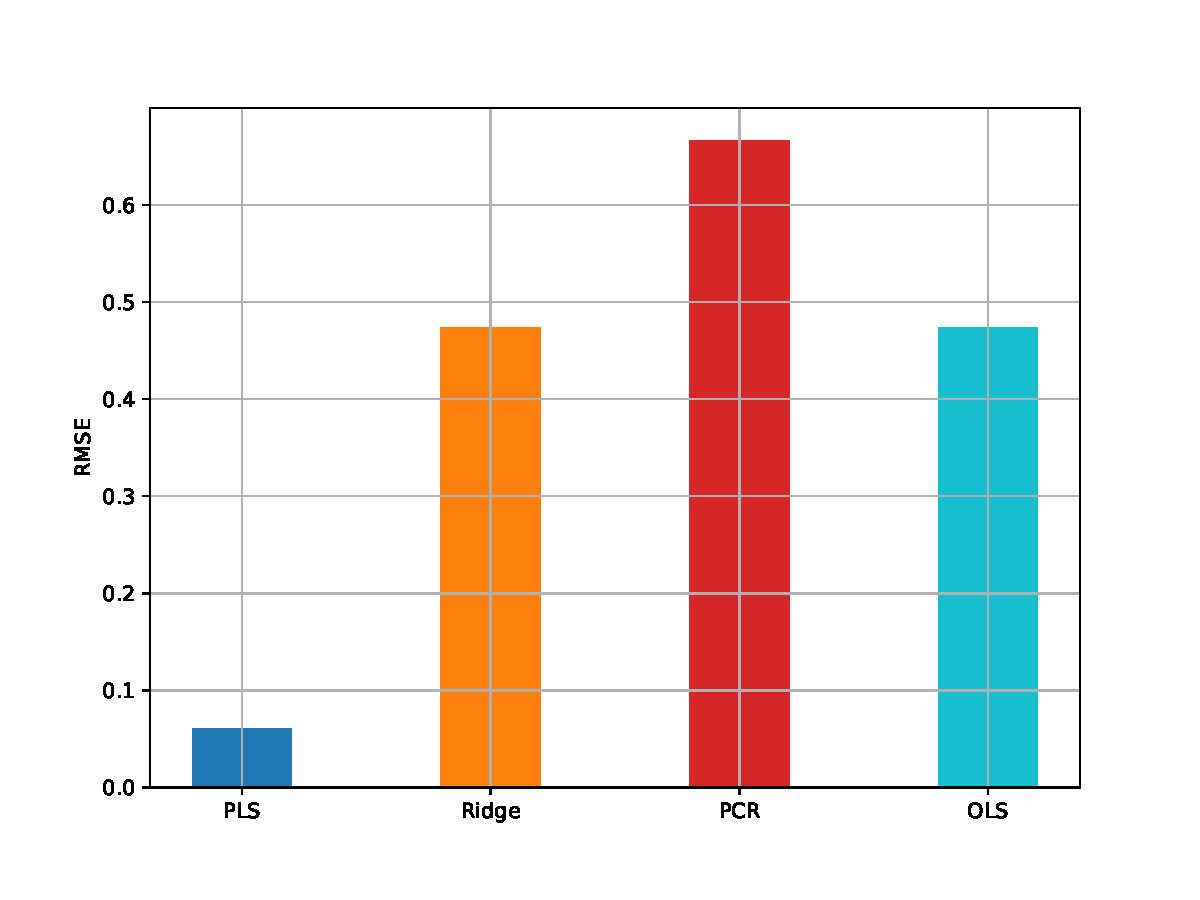
\includegraphics[width=0.5\textwidth]{../../code/hw2/figures/5-summary.pdf}}
  \caption{Best value for RMSE for the proposed approaches.}
  \label{fig:5-summary}
\end{figure}

The regression models RMSE is summarized in Fig.~\ref{fig:5-summary}. We present an extended result, where PCR+ and PCR- take in account 2 and 40 PCs, respectively. The same idea is applied for PLS+ and PLS-. 

The models: OLS, Ridge, PLS+ present a similar performance, with a low RMSE, with favorable $R^2$ values. As the number of components increase, both PLS and PCR improve the performance, however it impacts on the model performance. Moreover, both PCR+ and PCR- support that the regression is not suitable for the proposed problem since simpler solutions provide better results. 

\section{Conclusion}
Among the results obtained, there were no great differences between the results of the models, which favors the use of simpler models and lower computational cost, to the detriment of little improvement in prediction with the increase of cost. Therefore, unless there is a real need to obtain the best possible results, the most cost-effective solution was simple linear regression, since it is inexpensive and obtained results that were not much inferior to its peers. 

Nonetheless if computational cost is not taking in account, the best model for the given data set is the ridge regression model, since it presented the best results both in validation and in the test set.


\section*{Appendix}
% \vspace(-0 cm)
\begin{figure}[htbp!]
  \centerline{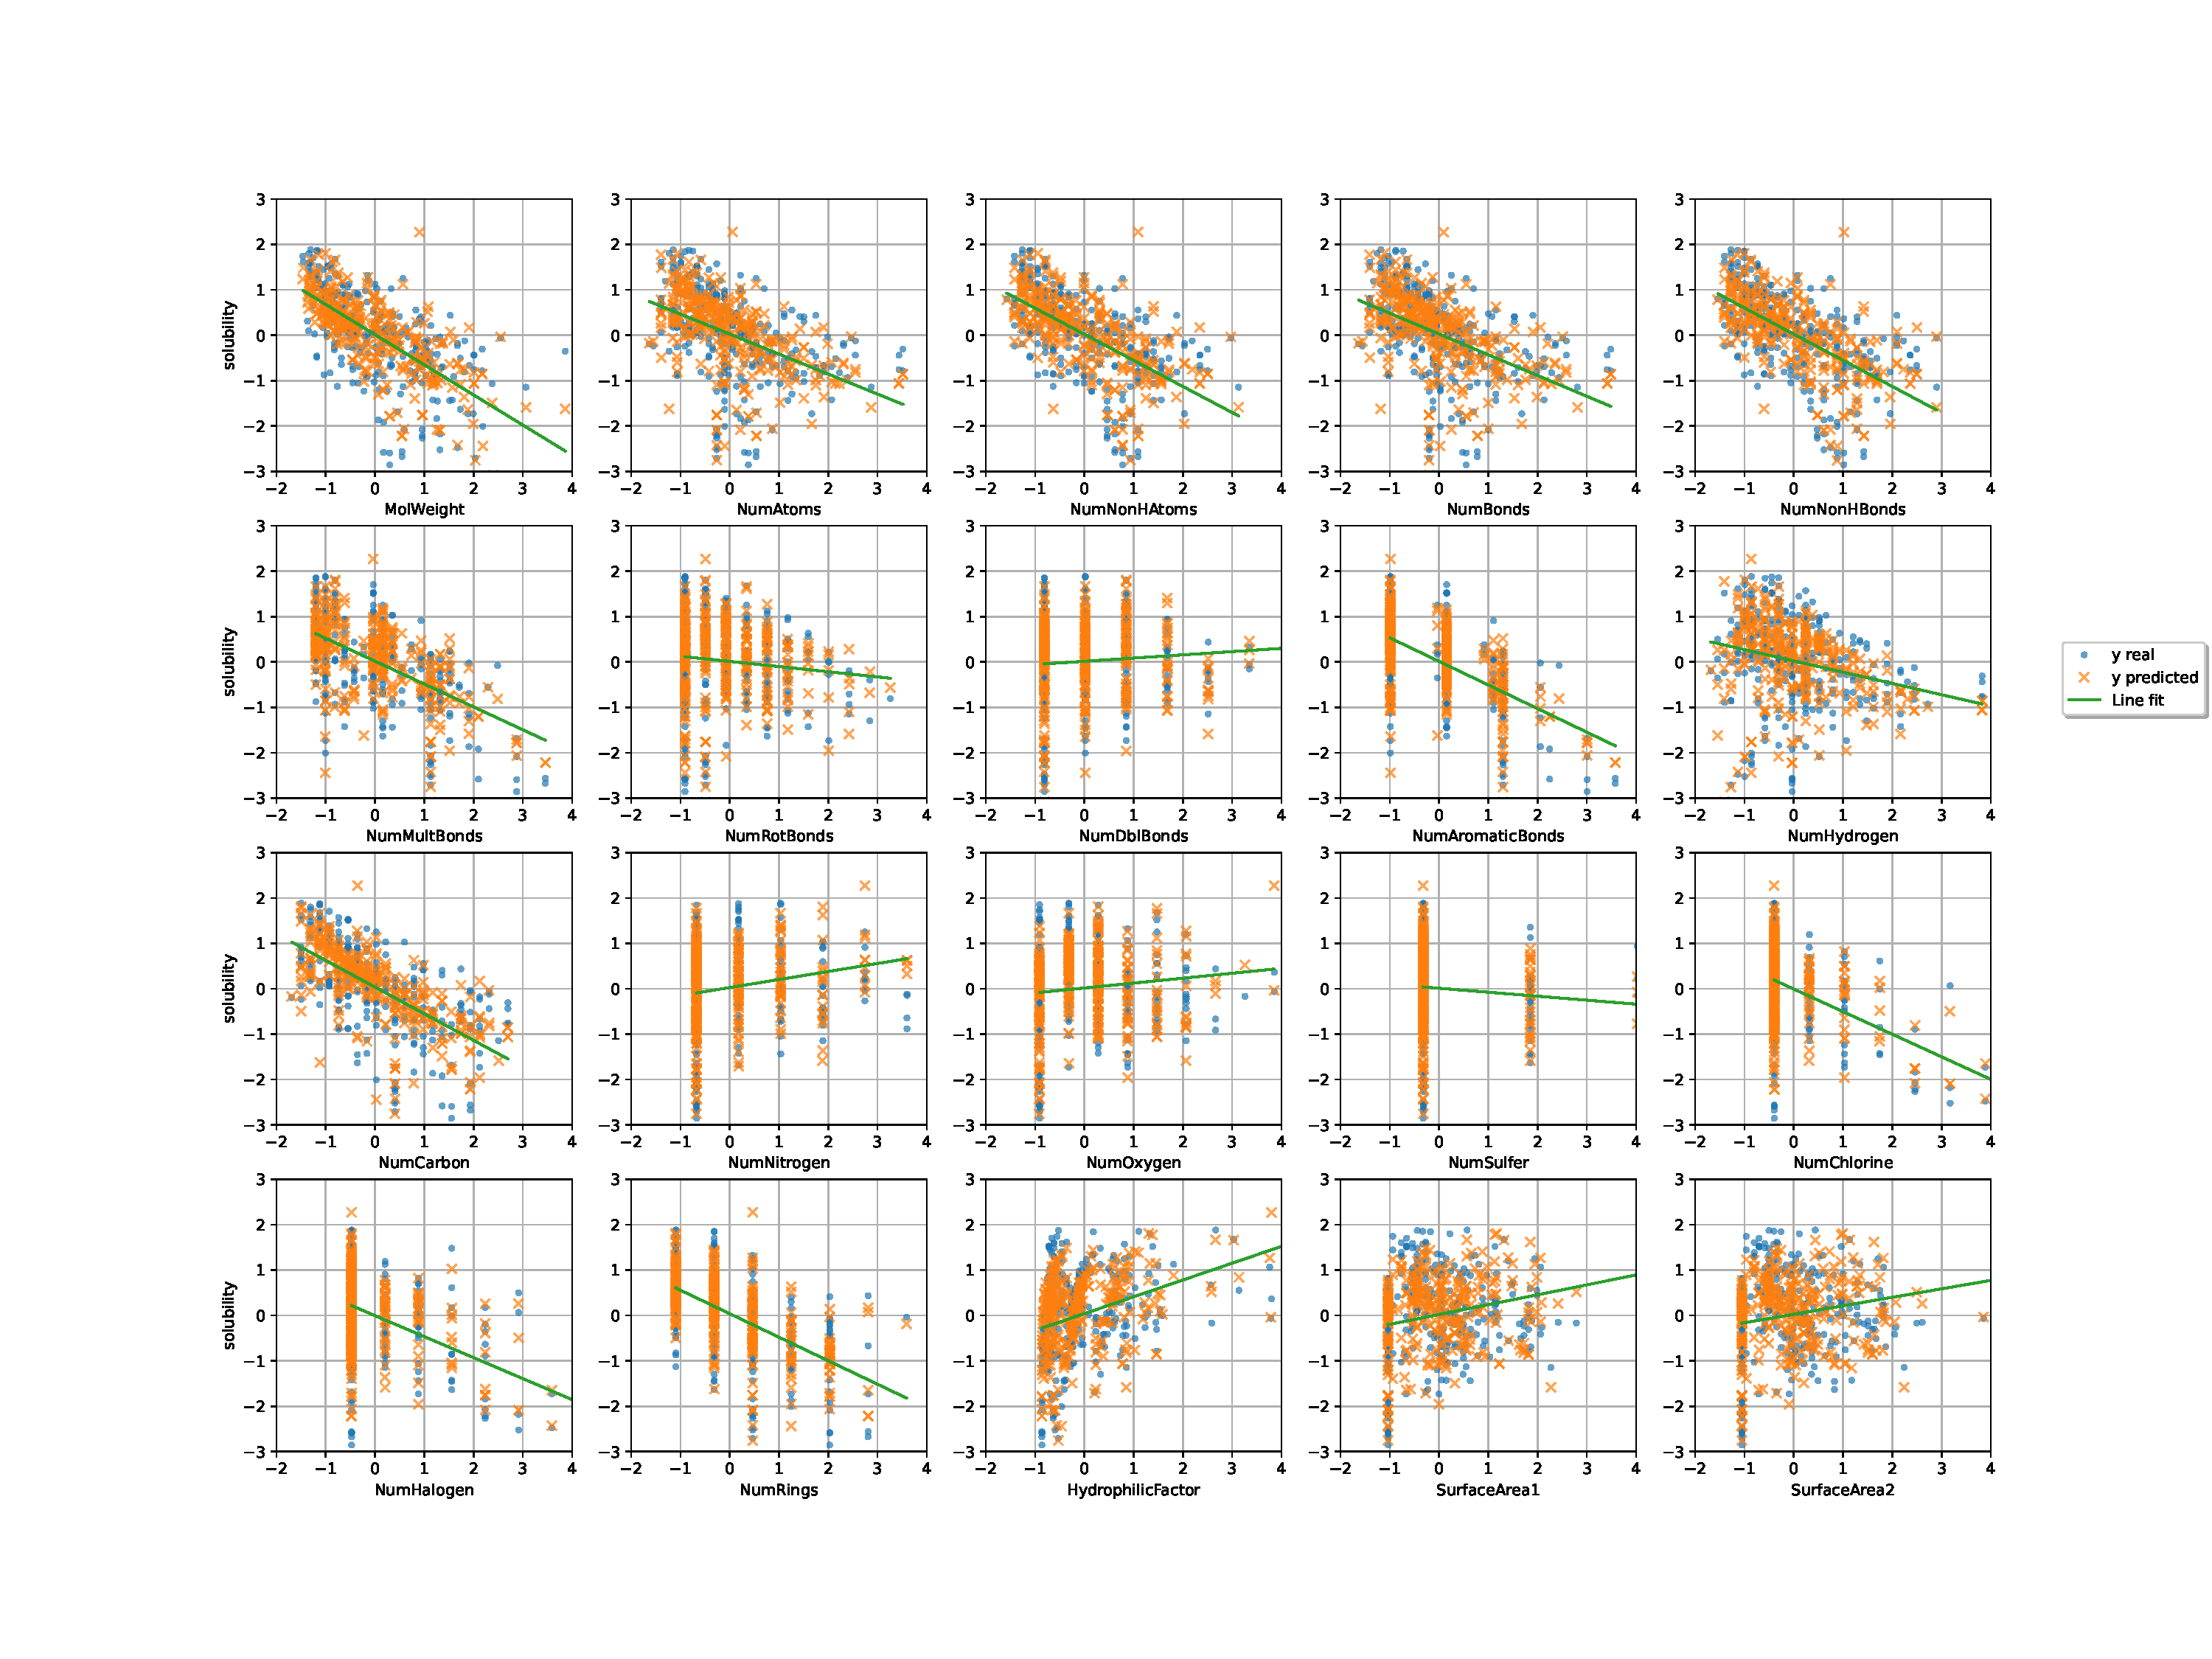
\includegraphics[width=0.5\textwidth]{../../code/hw2/figures/2-linear-regression.pdf}}
  \caption{Linear regression.}
  \label{fig:2-linear-regression}
\end{figure}

